\section{Kernel-Independent Fast Multipole Method}
If we consider a many body problem formed of $N$ potential/quadrature points $\{{\bm{y}}_n\}$ each with an associated potential/force $\{{\bm{f}}_n\}$ that we will evaluate on $M$ collocation points $\{\bm{x}_m\}$ then we can compute the velocity at each $\bm{x}_m$ where $m=1,2,\dots,M$ through
\begin{equation*}
    \bm{u}(\bm{x}) = \sum_{i=1}^N \Phi(\bm{x},{\bm{y}}_i){\bm{f}}_i
\end{equation*}
where $\Phi$ is the green's function associated with the underlying partial differential equation governing the dynamics of the system. In particular, $\Phi=S^\epsilon$ is our kernel for the case of the method of regularised Stokeslets where we compute the velocity of the fluid at a set of collocation points based on a set of body forces defined on solid boundaries within the fluid. This can be written as a matrix-vector product as described in \cref{eq:matrixvectorproduct}. This direct solution has a computational complexity of $\mathcal{O}(NM)$ which for either a large number of collocation points or quadrature points quickly becomes prohibitive due. In order to compute large systems we need to look at faster methods to approximate this vector-matrix product. One such set of methods is the familiy of fast multipole method's which can approximate \cref{eq:matrixvectorproduct} with complexity $\mathcal{O}(N+M)$. The standard fast multipole method (FMM) algorithm uses multipole expansion's of the kernel about the quadrature points in order to approximate long-range interaction between distant quadrature and target points \cite{Beatson,Tornberg2008,Wang2007AEquations,Yokota}. This method proves time-consuming to find for particular kernels such as regularised Stokeslets where the corresponding expansions first need to be computed by hand, it also means that the entire program is kernel dependent and any changes to the kernel need a complete recalculation of the expansions employed.
Instead we will look at an adaption to the FMM algorithm to create a kernel independent fast multipole algorithm (KIFMM) \cite{Ying2004, Ying2005,Rostami2016Kernel-independentStokeslets,Yan}. Using equivalent potentials instead of multipole expansions we can approximate long-range interactions using only kernel evaluations without computing every particle to particle interaction. This dramatically reduces the number of kernel evaluations compared to computation by the direct solution. 

\subsection{Hierarchical decomposition of the computational domain}
Both FMM and KIFMM are based on the Hierarchical decomposition of the computational domain. We let $\mathcal{D}$ be the computational domain, which we define to be a cube in $\mathcal{R}^3$ such that it encompasses all points in $\{\bm{y}_n\}$ and $\{\bm{x}_m\}$. We typically define this to be the smallest possible cube which includes all the points. The FMM method builds an Octree structure of cubes in 3D with the cube $\mathcal{D}$ as the root node. We will label this node the Level $0$ partition where no subdivision had occurred. Each subsequent division is made of $8$ equal-sized cubes each with a side length of half of the cube above. For each level, we subdivide a node into its $8$ children if the number of source points or target points within the cube is greater than some threshold $s\geq 1$. For efficiency only points of the type which exceed the threshold are moved from to the child nodes. This subdivision creates a new level $L+1$ containing the children of all subdivided nodes in level $L$. We refer to the node on level $L$ as the parent of nodes on level $L+1$. This process is repeated until all cubes have less than $s$ source or target points contained within them which we will refer to as leaf nodes.

\begin{figure}[ht]
    \centering
    \resizebox{.6\linewidth}{!}{% This file was created by matlab2tikz.
%
%The latest updates can be retrieved from
%  http://www.mathworks.com/matlabcentral/fileexchange/22022-matlab2tikz-matlab2tikz
%where you can also make suggestions and rate matlab2tikz.
%
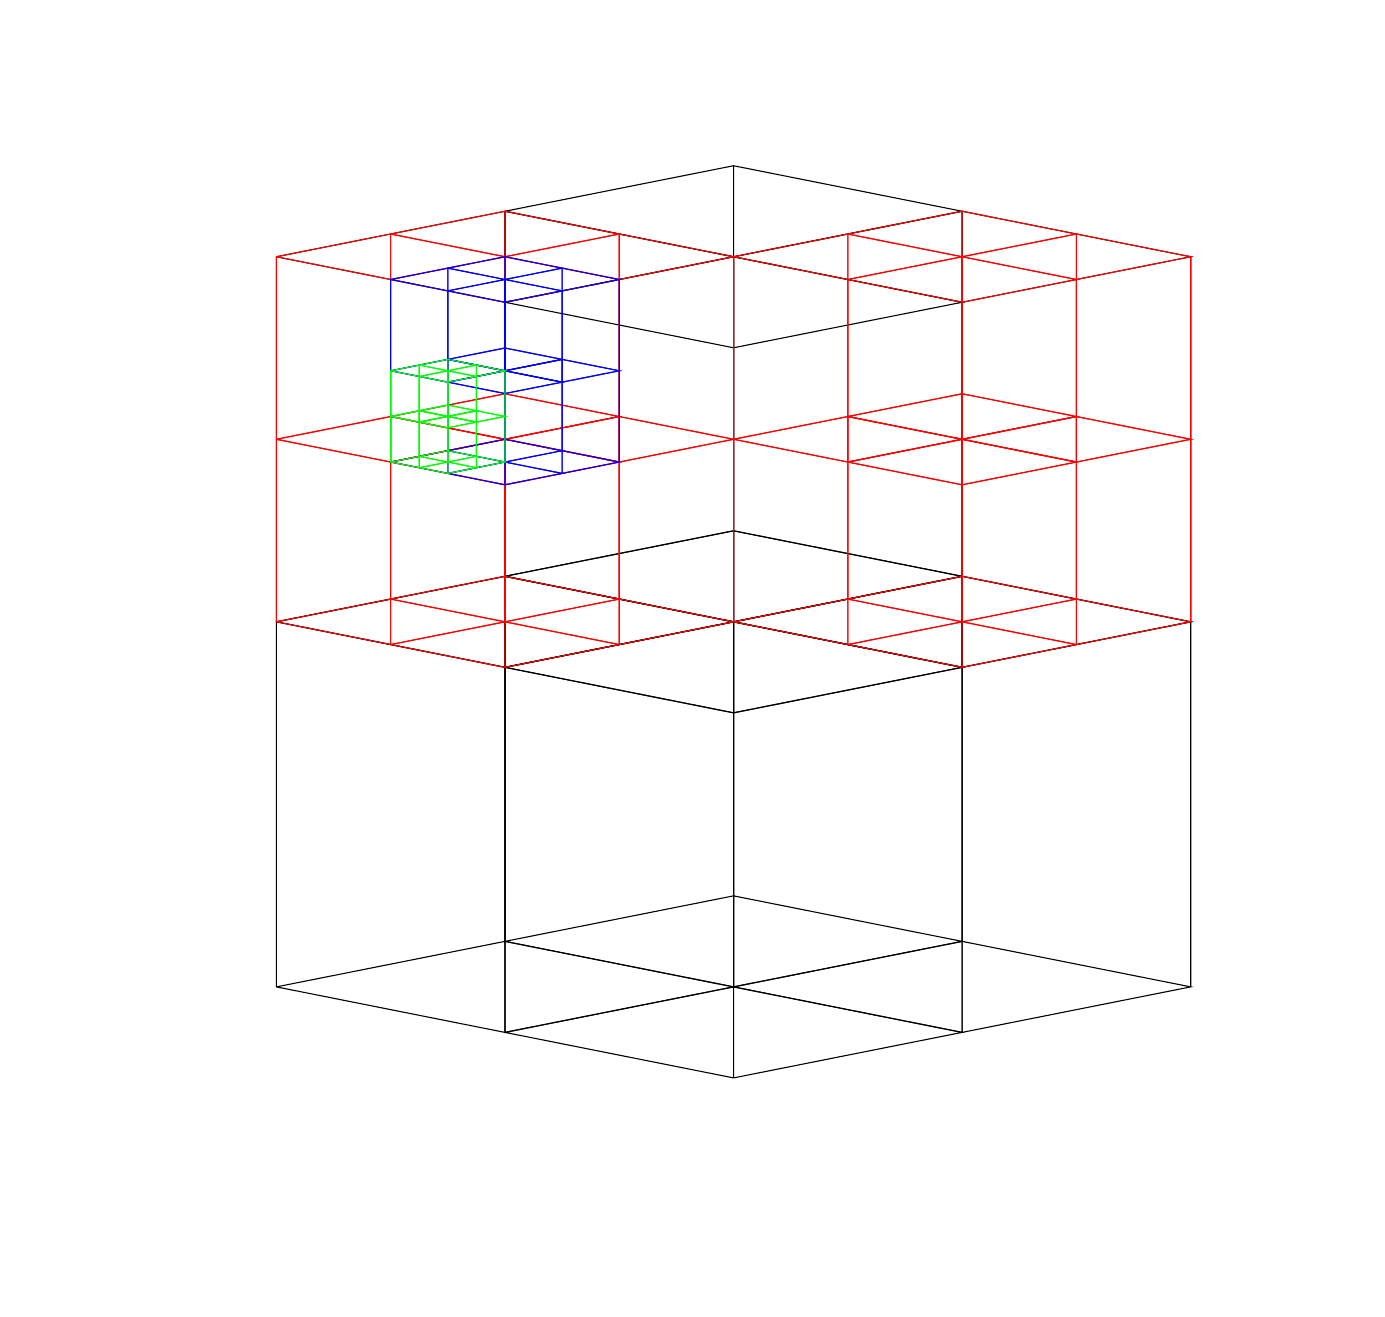
\begin{tikzpicture}

\begin{axis}[%
width=5.151in,
height=5.139in,
at={(0.864in,0.694in)},
scale only axis,
unbounded coords=jump,
xmin=0,
xmax=1,
tick align=outside,
ymin=0,
ymax=1,
zmin=0,
zmax=1,
view={45}{10},
axis line style={draw=none},
ticks=none,
axis x line*=bottom,
axis y line*=left,
axis z line*=left
]
\addplot3 [color=black]
 table[row sep=crcr] {%
0.0737015537421595	0.0737015537421595	0.0737015537421595\\
0.517448266926349	0.0737015537421595	0.0737015537421595\\
0.517448266926349	0.517448266926349	0.0737015537421595\\
0.0737015537421595	0.517448266926349	0.0737015537421595\\
0.0737015537421595	0.0737015537421595	0.0737015537421595\\
0.0737015537421595	0.0737015537421595	0.517448266926349\\
0.517448266926349	0.0737015537421595	0.517448266926349\\
0.517448266926349	0.517448266926349	0.517448266926349\\
0.0737015537421595	0.517448266926349	0.517448266926349\\
0.0737015537421595	0.0737015537421595	0.517448266926349\\
0.0737015537421595	0.0737015537421595	0.0737015537421595\\
nan	nan	nan\\
0.517448266926349	0.0737015537421595	0.0737015537421595\\
0.517448266926349	0.0737015537421595	0.517448266926349\\
nan	nan	nan\\
0.517448266926349	0.517448266926349	0.0737015537421595\\
0.517448266926349	0.517448266926349	0.517448266926349\\
nan	nan	nan\\
0.0737015537421595	0.517448266926349	0.0737015537421595\\
0.0737015537421595	0.517448266926349	0.517448266926349\\
};
 \addplot3 [color=black]
 table[row sep=crcr] {%
0.0737015537421595	0.0737015537421595	0.517448266926349\\
0.517448266926349	0.0737015537421595	0.517448266926349\\
0.517448266926349	0.517448266926349	0.517448266926349\\
0.0737015537421595	0.517448266926349	0.517448266926349\\
0.0737015537421595	0.0737015537421595	0.517448266926349\\
0.0737015537421595	0.0737015537421595	0.961194980110539\\
0.517448266926349	0.0737015537421595	0.961194980110539\\
0.517448266926349	0.517448266926349	0.961194980110539\\
0.0737015537421595	0.517448266926349	0.961194980110539\\
0.0737015537421595	0.0737015537421595	0.961194980110539\\
0.0737015537421595	0.0737015537421595	0.517448266926349\\
nan	nan	nan\\
0.517448266926349	0.0737015537421595	0.517448266926349\\
0.517448266926349	0.0737015537421595	0.961194980110539\\
nan	nan	nan\\
0.517448266926349	0.517448266926349	0.517448266926349\\
0.517448266926349	0.517448266926349	0.961194980110539\\
nan	nan	nan\\
0.0737015537421595	0.517448266926349	0.517448266926349\\
0.0737015537421595	0.517448266926349	0.961194980110539\\
};
 \addplot3 [color=black]
 table[row sep=crcr] {%
0.0737015537421595	0.517448266926349	0.0737015537421595\\
0.517448266926349	0.517448266926349	0.0737015537421595\\
0.517448266926349	0.961194980110539	0.0737015537421595\\
0.0737015537421595	0.961194980110539	0.0737015537421595\\
0.0737015537421595	0.517448266926349	0.0737015537421595\\
0.0737015537421595	0.517448266926349	0.517448266926349\\
0.517448266926349	0.517448266926349	0.517448266926349\\
0.517448266926349	0.961194980110539	0.517448266926349\\
0.0737015537421595	0.961194980110539	0.517448266926349\\
0.0737015537421595	0.517448266926349	0.517448266926349\\
0.0737015537421595	0.517448266926349	0.0737015537421595\\
nan	nan	nan\\
0.517448266926349	0.517448266926349	0.0737015537421595\\
0.517448266926349	0.517448266926349	0.517448266926349\\
nan	nan	nan\\
0.517448266926349	0.961194980110539	0.0737015537421595\\
0.517448266926349	0.961194980110539	0.517448266926349\\
nan	nan	nan\\
0.0737015537421595	0.961194980110539	0.0737015537421595\\
0.0737015537421595	0.961194980110539	0.517448266926349\\
};
 \addplot3 [color=black]
 table[row sep=crcr] {%
0.0737015537421595	0.517448266926349	0.517448266926349\\
0.517448266926349	0.517448266926349	0.517448266926349\\
0.517448266926349	0.961194980110539	0.517448266926349\\
0.0737015537421595	0.961194980110539	0.517448266926349\\
0.0737015537421595	0.517448266926349	0.517448266926349\\
0.0737015537421595	0.517448266926349	0.961194980110539\\
0.517448266926349	0.517448266926349	0.961194980110539\\
0.517448266926349	0.961194980110539	0.961194980110539\\
0.0737015537421595	0.961194980110539	0.961194980110539\\
0.0737015537421595	0.517448266926349	0.961194980110539\\
0.0737015537421595	0.517448266926349	0.517448266926349\\
nan	nan	nan\\
0.517448266926349	0.517448266926349	0.517448266926349\\
0.517448266926349	0.517448266926349	0.961194980110539\\
nan	nan	nan\\
0.517448266926349	0.961194980110539	0.517448266926349\\
0.517448266926349	0.961194980110539	0.961194980110539\\
nan	nan	nan\\
0.0737015537421595	0.961194980110539	0.517448266926349\\
0.0737015537421595	0.961194980110539	0.961194980110539\\
};
 \addplot3 [color=black]
 table[row sep=crcr] {%
0.517448266926349	0.0737015537421595	0.0737015537421595\\
0.961194980110539	0.0737015537421595	0.0737015537421595\\
0.961194980110539	0.517448266926349	0.0737015537421595\\
0.517448266926349	0.517448266926349	0.0737015537421595\\
0.517448266926349	0.0737015537421595	0.0737015537421595\\
0.517448266926349	0.0737015537421595	0.517448266926349\\
0.961194980110539	0.0737015537421595	0.517448266926349\\
0.961194980110539	0.517448266926349	0.517448266926349\\
0.517448266926349	0.517448266926349	0.517448266926349\\
0.517448266926349	0.0737015537421595	0.517448266926349\\
0.517448266926349	0.0737015537421595	0.0737015537421595\\
nan	nan	nan\\
0.961194980110539	0.0737015537421595	0.0737015537421595\\
0.961194980110539	0.0737015537421595	0.517448266926349\\
nan	nan	nan\\
0.961194980110539	0.517448266926349	0.0737015537421595\\
0.961194980110539	0.517448266926349	0.517448266926349\\
nan	nan	nan\\
0.517448266926349	0.517448266926349	0.0737015537421595\\
0.517448266926349	0.517448266926349	0.517448266926349\\
};
 \addplot3 [color=black]
 table[row sep=crcr] {%
0.517448266926349	0.0737015537421595	0.517448266926349\\
0.961194980110539	0.0737015537421595	0.517448266926349\\
0.961194980110539	0.517448266926349	0.517448266926349\\
0.517448266926349	0.517448266926349	0.517448266926349\\
0.517448266926349	0.0737015537421595	0.517448266926349\\
0.517448266926349	0.0737015537421595	0.961194980110539\\
0.961194980110539	0.0737015537421595	0.961194980110539\\
0.961194980110539	0.517448266926349	0.961194980110539\\
0.517448266926349	0.517448266926349	0.961194980110539\\
0.517448266926349	0.0737015537421595	0.961194980110539\\
0.517448266926349	0.0737015537421595	0.517448266926349\\
nan	nan	nan\\
0.961194980110539	0.0737015537421595	0.517448266926349\\
0.961194980110539	0.0737015537421595	0.961194980110539\\
nan	nan	nan\\
0.961194980110539	0.517448266926349	0.517448266926349\\
0.961194980110539	0.517448266926349	0.961194980110539\\
nan	nan	nan\\
0.517448266926349	0.517448266926349	0.517448266926349\\
0.517448266926349	0.517448266926349	0.961194980110539\\
};
 \addplot3 [color=black]
 table[row sep=crcr] {%
0.517448266926349	0.517448266926349	0.0737015537421595\\
0.961194980110539	0.517448266926349	0.0737015537421595\\
0.961194980110539	0.961194980110539	0.0737015537421595\\
0.517448266926349	0.961194980110539	0.0737015537421595\\
0.517448266926349	0.517448266926349	0.0737015537421595\\
0.517448266926349	0.517448266926349	0.517448266926349\\
0.961194980110539	0.517448266926349	0.517448266926349\\
0.961194980110539	0.961194980110539	0.517448266926349\\
0.517448266926349	0.961194980110539	0.517448266926349\\
0.517448266926349	0.517448266926349	0.517448266926349\\
0.517448266926349	0.517448266926349	0.0737015537421595\\
nan	nan	nan\\
0.961194980110539	0.517448266926349	0.0737015537421595\\
0.961194980110539	0.517448266926349	0.517448266926349\\
nan	nan	nan\\
0.961194980110539	0.961194980110539	0.0737015537421595\\
0.961194980110539	0.961194980110539	0.517448266926349\\
nan	nan	nan\\
0.517448266926349	0.961194980110539	0.0737015537421595\\
0.517448266926349	0.961194980110539	0.517448266926349\\
};
 \addplot3 [color=black]
 table[row sep=crcr] {%
0.517448266926349	0.517448266926349	0.517448266926349\\
0.961194980110539	0.517448266926349	0.517448266926349\\
0.961194980110539	0.961194980110539	0.517448266926349\\
0.517448266926349	0.961194980110539	0.517448266926349\\
0.517448266926349	0.517448266926349	0.517448266926349\\
0.517448266926349	0.517448266926349	0.961194980110539\\
0.961194980110539	0.517448266926349	0.961194980110539\\
0.961194980110539	0.961194980110539	0.961194980110539\\
0.517448266926349	0.961194980110539	0.961194980110539\\
0.517448266926349	0.517448266926349	0.961194980110539\\
0.517448266926349	0.517448266926349	0.517448266926349\\
nan	nan	nan\\
0.961194980110539	0.517448266926349	0.517448266926349\\
0.961194980110539	0.517448266926349	0.961194980110539\\
nan	nan	nan\\
0.961194980110539	0.961194980110539	0.517448266926349\\
0.961194980110539	0.961194980110539	0.961194980110539\\
nan	nan	nan\\
0.517448266926349	0.961194980110539	0.517448266926349\\
0.517448266926349	0.961194980110539	0.961194980110539\\
};
 \addplot3 [color=red]
 table[row sep=crcr] {%
0.0737015537421595	0.0737015537421595	0.517448266926349\\
0.295574910334254	0.0737015537421595	0.517448266926349\\
0.295574910334254	0.295574910334254	0.517448266926349\\
0.0737015537421595	0.295574910334254	0.517448266926349\\
0.0737015537421595	0.0737015537421595	0.517448266926349\\
0.0737015537421595	0.0737015537421595	0.739321623518444\\
0.295574910334254	0.0737015537421595	0.739321623518444\\
0.295574910334254	0.295574910334254	0.739321623518444\\
0.0737015537421595	0.295574910334254	0.739321623518444\\
0.0737015537421595	0.0737015537421595	0.739321623518444\\
0.0737015537421595	0.0737015537421595	0.517448266926349\\
nan	nan	nan\\
0.295574910334254	0.0737015537421595	0.517448266926349\\
0.295574910334254	0.0737015537421595	0.739321623518444\\
nan	nan	nan\\
0.295574910334254	0.295574910334254	0.517448266926349\\
0.295574910334254	0.295574910334254	0.739321623518444\\
nan	nan	nan\\
0.0737015537421595	0.295574910334254	0.517448266926349\\
0.0737015537421595	0.295574910334254	0.739321623518444\\
};
 \addplot3 [color=red]
 table[row sep=crcr] {%
0.0737015537421595	0.0737015537421595	0.739321623518444\\
0.295574910334254	0.0737015537421595	0.739321623518444\\
0.295574910334254	0.295574910334254	0.739321623518444\\
0.0737015537421595	0.295574910334254	0.739321623518444\\
0.0737015537421595	0.0737015537421595	0.739321623518444\\
0.0737015537421595	0.0737015537421595	0.961194980110539\\
0.295574910334254	0.0737015537421595	0.961194980110539\\
0.295574910334254	0.295574910334254	0.961194980110539\\
0.0737015537421595	0.295574910334254	0.961194980110539\\
0.0737015537421595	0.0737015537421595	0.961194980110539\\
0.0737015537421595	0.0737015537421595	0.739321623518444\\
nan	nan	nan\\
0.295574910334254	0.0737015537421595	0.739321623518444\\
0.295574910334254	0.0737015537421595	0.961194980110539\\
nan	nan	nan\\
0.295574910334254	0.295574910334254	0.739321623518444\\
0.295574910334254	0.295574910334254	0.961194980110539\\
nan	nan	nan\\
0.0737015537421595	0.295574910334254	0.739321623518444\\
0.0737015537421595	0.295574910334254	0.961194980110539\\
};
 \addplot3 [color=red]
 table[row sep=crcr] {%
0.0737015537421595	0.295574910334254	0.517448266926349\\
0.295574910334254	0.295574910334254	0.517448266926349\\
0.295574910334254	0.517448266926349	0.517448266926349\\
0.0737015537421595	0.517448266926349	0.517448266926349\\
0.0737015537421595	0.295574910334254	0.517448266926349\\
0.0737015537421595	0.295574910334254	0.739321623518444\\
0.295574910334254	0.295574910334254	0.739321623518444\\
0.295574910334254	0.517448266926349	0.739321623518444\\
0.0737015537421595	0.517448266926349	0.739321623518444\\
0.0737015537421595	0.295574910334254	0.739321623518444\\
0.0737015537421595	0.295574910334254	0.517448266926349\\
nan	nan	nan\\
0.295574910334254	0.295574910334254	0.517448266926349\\
0.295574910334254	0.295574910334254	0.739321623518444\\
nan	nan	nan\\
0.295574910334254	0.517448266926349	0.517448266926349\\
0.295574910334254	0.517448266926349	0.739321623518444\\
nan	nan	nan\\
0.0737015537421595	0.517448266926349	0.517448266926349\\
0.0737015537421595	0.517448266926349	0.739321623518444\\
};
 \addplot3 [color=red]
 table[row sep=crcr] {%
0.0737015537421595	0.295574910334254	0.739321623518444\\
0.295574910334254	0.295574910334254	0.739321623518444\\
0.295574910334254	0.517448266926349	0.739321623518444\\
0.0737015537421595	0.517448266926349	0.739321623518444\\
0.0737015537421595	0.295574910334254	0.739321623518444\\
0.0737015537421595	0.295574910334254	0.961194980110539\\
0.295574910334254	0.295574910334254	0.961194980110539\\
0.295574910334254	0.517448266926349	0.961194980110539\\
0.0737015537421595	0.517448266926349	0.961194980110539\\
0.0737015537421595	0.295574910334254	0.961194980110539\\
0.0737015537421595	0.295574910334254	0.739321623518444\\
nan	nan	nan\\
0.295574910334254	0.295574910334254	0.739321623518444\\
0.295574910334254	0.295574910334254	0.961194980110539\\
nan	nan	nan\\
0.295574910334254	0.517448266926349	0.739321623518444\\
0.295574910334254	0.517448266926349	0.961194980110539\\
nan	nan	nan\\
0.0737015537421595	0.517448266926349	0.739321623518444\\
0.0737015537421595	0.517448266926349	0.961194980110539\\
};
 \addplot3 [color=red]
 table[row sep=crcr] {%
0.295574910334254	0.0737015537421595	0.517448266926349\\
0.517448266926349	0.0737015537421595	0.517448266926349\\
0.517448266926349	0.295574910334254	0.517448266926349\\
0.295574910334254	0.295574910334254	0.517448266926349\\
0.295574910334254	0.0737015537421595	0.517448266926349\\
0.295574910334254	0.0737015537421595	0.739321623518444\\
0.517448266926349	0.0737015537421595	0.739321623518444\\
0.517448266926349	0.295574910334254	0.739321623518444\\
0.295574910334254	0.295574910334254	0.739321623518444\\
0.295574910334254	0.0737015537421595	0.739321623518444\\
0.295574910334254	0.0737015537421595	0.517448266926349\\
nan	nan	nan\\
0.517448266926349	0.0737015537421595	0.517448266926349\\
0.517448266926349	0.0737015537421595	0.739321623518444\\
nan	nan	nan\\
0.517448266926349	0.295574910334254	0.517448266926349\\
0.517448266926349	0.295574910334254	0.739321623518444\\
nan	nan	nan\\
0.295574910334254	0.295574910334254	0.517448266926349\\
0.295574910334254	0.295574910334254	0.739321623518444\\
};
 \addplot3 [color=red]
 table[row sep=crcr] {%
0.295574910334254	0.0737015537421595	0.739321623518444\\
0.517448266926349	0.0737015537421595	0.739321623518444\\
0.517448266926349	0.295574910334254	0.739321623518444\\
0.295574910334254	0.295574910334254	0.739321623518444\\
0.295574910334254	0.0737015537421595	0.739321623518444\\
0.295574910334254	0.0737015537421595	0.961194980110539\\
0.517448266926349	0.0737015537421595	0.961194980110539\\
0.517448266926349	0.295574910334254	0.961194980110539\\
0.295574910334254	0.295574910334254	0.961194980110539\\
0.295574910334254	0.0737015537421595	0.961194980110539\\
0.295574910334254	0.0737015537421595	0.739321623518444\\
nan	nan	nan\\
0.517448266926349	0.0737015537421595	0.739321623518444\\
0.517448266926349	0.0737015537421595	0.961194980110539\\
nan	nan	nan\\
0.517448266926349	0.295574910334254	0.739321623518444\\
0.517448266926349	0.295574910334254	0.961194980110539\\
nan	nan	nan\\
0.295574910334254	0.295574910334254	0.739321623518444\\
0.295574910334254	0.295574910334254	0.961194980110539\\
};
 \addplot3 [color=red]
 table[row sep=crcr] {%
0.295574910334254	0.295574910334254	0.517448266926349\\
0.517448266926349	0.295574910334254	0.517448266926349\\
0.517448266926349	0.517448266926349	0.517448266926349\\
0.295574910334254	0.517448266926349	0.517448266926349\\
0.295574910334254	0.295574910334254	0.517448266926349\\
0.295574910334254	0.295574910334254	0.739321623518444\\
0.517448266926349	0.295574910334254	0.739321623518444\\
0.517448266926349	0.517448266926349	0.739321623518444\\
0.295574910334254	0.517448266926349	0.739321623518444\\
0.295574910334254	0.295574910334254	0.739321623518444\\
0.295574910334254	0.295574910334254	0.517448266926349\\
nan	nan	nan\\
0.517448266926349	0.295574910334254	0.517448266926349\\
0.517448266926349	0.295574910334254	0.739321623518444\\
nan	nan	nan\\
0.517448266926349	0.517448266926349	0.517448266926349\\
0.517448266926349	0.517448266926349	0.739321623518444\\
nan	nan	nan\\
0.295574910334254	0.517448266926349	0.517448266926349\\
0.295574910334254	0.517448266926349	0.739321623518444\\
};
 \addplot3 [color=red]
 table[row sep=crcr] {%
0.295574910334254	0.295574910334254	0.739321623518444\\
0.517448266926349	0.295574910334254	0.739321623518444\\
0.517448266926349	0.517448266926349	0.739321623518444\\
0.295574910334254	0.517448266926349	0.739321623518444\\
0.295574910334254	0.295574910334254	0.739321623518444\\
0.295574910334254	0.295574910334254	0.961194980110539\\
0.517448266926349	0.295574910334254	0.961194980110539\\
0.517448266926349	0.517448266926349	0.961194980110539\\
0.295574910334254	0.517448266926349	0.961194980110539\\
0.295574910334254	0.295574910334254	0.961194980110539\\
0.295574910334254	0.295574910334254	0.739321623518444\\
nan	nan	nan\\
0.517448266926349	0.295574910334254	0.739321623518444\\
0.517448266926349	0.295574910334254	0.961194980110539\\
nan	nan	nan\\
0.517448266926349	0.517448266926349	0.739321623518444\\
0.517448266926349	0.517448266926349	0.961194980110539\\
nan	nan	nan\\
0.295574910334254	0.517448266926349	0.739321623518444\\
0.295574910334254	0.517448266926349	0.961194980110539\\
};
 \addplot3 [color=red]
 table[row sep=crcr] {%
0.517448266926349	0.517448266926349	0.517448266926349\\
0.739321623518444	0.517448266926349	0.517448266926349\\
0.739321623518444	0.739321623518444	0.517448266926349\\
0.517448266926349	0.739321623518444	0.517448266926349\\
0.517448266926349	0.517448266926349	0.517448266926349\\
0.517448266926349	0.517448266926349	0.739321623518444\\
0.739321623518444	0.517448266926349	0.739321623518444\\
0.739321623518444	0.739321623518444	0.739321623518444\\
0.517448266926349	0.739321623518444	0.739321623518444\\
0.517448266926349	0.517448266926349	0.739321623518444\\
0.517448266926349	0.517448266926349	0.517448266926349\\
nan	nan	nan\\
0.739321623518444	0.517448266926349	0.517448266926349\\
0.739321623518444	0.517448266926349	0.739321623518444\\
nan	nan	nan\\
0.739321623518444	0.739321623518444	0.517448266926349\\
0.739321623518444	0.739321623518444	0.739321623518444\\
nan	nan	nan\\
0.517448266926349	0.739321623518444	0.517448266926349\\
0.517448266926349	0.739321623518444	0.739321623518444\\
};
 \addplot3 [color=red]
 table[row sep=crcr] {%
0.517448266926349	0.517448266926349	0.739321623518444\\
0.739321623518444	0.517448266926349	0.739321623518444\\
0.739321623518444	0.739321623518444	0.739321623518444\\
0.517448266926349	0.739321623518444	0.739321623518444\\
0.517448266926349	0.517448266926349	0.739321623518444\\
0.517448266926349	0.517448266926349	0.961194980110539\\
0.739321623518444	0.517448266926349	0.961194980110539\\
0.739321623518444	0.739321623518444	0.961194980110539\\
0.517448266926349	0.739321623518444	0.961194980110539\\
0.517448266926349	0.517448266926349	0.961194980110539\\
0.517448266926349	0.517448266926349	0.739321623518444\\
nan	nan	nan\\
0.739321623518444	0.517448266926349	0.739321623518444\\
0.739321623518444	0.517448266926349	0.961194980110539\\
nan	nan	nan\\
0.739321623518444	0.739321623518444	0.739321623518444\\
0.739321623518444	0.739321623518444	0.961194980110539\\
nan	nan	nan\\
0.517448266926349	0.739321623518444	0.739321623518444\\
0.517448266926349	0.739321623518444	0.961194980110539\\
};
 \addplot3 [color=red]
 table[row sep=crcr] {%
0.517448266926349	0.739321623518444	0.517448266926349\\
0.739321623518444	0.739321623518444	0.517448266926349\\
0.739321623518444	0.961194980110539	0.517448266926349\\
0.517448266926349	0.961194980110539	0.517448266926349\\
0.517448266926349	0.739321623518444	0.517448266926349\\
0.517448266926349	0.739321623518444	0.739321623518444\\
0.739321623518444	0.739321623518444	0.739321623518444\\
0.739321623518444	0.961194980110539	0.739321623518444\\
0.517448266926349	0.961194980110539	0.739321623518444\\
0.517448266926349	0.739321623518444	0.739321623518444\\
0.517448266926349	0.739321623518444	0.517448266926349\\
nan	nan	nan\\
0.739321623518444	0.739321623518444	0.517448266926349\\
0.739321623518444	0.739321623518444	0.739321623518444\\
nan	nan	nan\\
0.739321623518444	0.961194980110539	0.517448266926349\\
0.739321623518444	0.961194980110539	0.739321623518444\\
nan	nan	nan\\
0.517448266926349	0.961194980110539	0.517448266926349\\
0.517448266926349	0.961194980110539	0.739321623518444\\
};
 \addplot3 [color=red]
 table[row sep=crcr] {%
0.517448266926349	0.739321623518444	0.739321623518444\\
0.739321623518444	0.739321623518444	0.739321623518444\\
0.739321623518444	0.961194980110539	0.739321623518444\\
0.517448266926349	0.961194980110539	0.739321623518444\\
0.517448266926349	0.739321623518444	0.739321623518444\\
0.517448266926349	0.739321623518444	0.961194980110539\\
0.739321623518444	0.739321623518444	0.961194980110539\\
0.739321623518444	0.961194980110539	0.961194980110539\\
0.517448266926349	0.961194980110539	0.961194980110539\\
0.517448266926349	0.739321623518444	0.961194980110539\\
0.517448266926349	0.739321623518444	0.739321623518444\\
nan	nan	nan\\
0.739321623518444	0.739321623518444	0.739321623518444\\
0.739321623518444	0.739321623518444	0.961194980110539\\
nan	nan	nan\\
0.739321623518444	0.961194980110539	0.739321623518444\\
0.739321623518444	0.961194980110539	0.961194980110539\\
nan	nan	nan\\
0.517448266926349	0.961194980110539	0.739321623518444\\
0.517448266926349	0.961194980110539	0.961194980110539\\
};
 \addplot3 [color=red]
 table[row sep=crcr] {%
0.739321623518444	0.517448266926349	0.517448266926349\\
0.961194980110539	0.517448266926349	0.517448266926349\\
0.961194980110539	0.739321623518444	0.517448266926349\\
0.739321623518444	0.739321623518444	0.517448266926349\\
0.739321623518444	0.517448266926349	0.517448266926349\\
0.739321623518444	0.517448266926349	0.739321623518444\\
0.961194980110539	0.517448266926349	0.739321623518444\\
0.961194980110539	0.739321623518444	0.739321623518444\\
0.739321623518444	0.739321623518444	0.739321623518444\\
0.739321623518444	0.517448266926349	0.739321623518444\\
0.739321623518444	0.517448266926349	0.517448266926349\\
nan	nan	nan\\
0.961194980110539	0.517448266926349	0.517448266926349\\
0.961194980110539	0.517448266926349	0.739321623518444\\
nan	nan	nan\\
0.961194980110539	0.739321623518444	0.517448266926349\\
0.961194980110539	0.739321623518444	0.739321623518444\\
nan	nan	nan\\
0.739321623518444	0.739321623518444	0.517448266926349\\
0.739321623518444	0.739321623518444	0.739321623518444\\
};
 \addplot3 [color=red]
 table[row sep=crcr] {%
0.739321623518444	0.517448266926349	0.739321623518444\\
0.961194980110539	0.517448266926349	0.739321623518444\\
0.961194980110539	0.739321623518444	0.739321623518444\\
0.739321623518444	0.739321623518444	0.739321623518444\\
0.739321623518444	0.517448266926349	0.739321623518444\\
0.739321623518444	0.517448266926349	0.961194980110539\\
0.961194980110539	0.517448266926349	0.961194980110539\\
0.961194980110539	0.739321623518444	0.961194980110539\\
0.739321623518444	0.739321623518444	0.961194980110539\\
0.739321623518444	0.517448266926349	0.961194980110539\\
0.739321623518444	0.517448266926349	0.739321623518444\\
nan	nan	nan\\
0.961194980110539	0.517448266926349	0.739321623518444\\
0.961194980110539	0.517448266926349	0.961194980110539\\
nan	nan	nan\\
0.961194980110539	0.739321623518444	0.739321623518444\\
0.961194980110539	0.739321623518444	0.961194980110539\\
nan	nan	nan\\
0.739321623518444	0.739321623518444	0.739321623518444\\
0.739321623518444	0.739321623518444	0.961194980110539\\
};
 \addplot3 [color=red]
 table[row sep=crcr] {%
0.739321623518444	0.739321623518444	0.517448266926349\\
0.961194980110539	0.739321623518444	0.517448266926349\\
0.961194980110539	0.961194980110539	0.517448266926349\\
0.739321623518444	0.961194980110539	0.517448266926349\\
0.739321623518444	0.739321623518444	0.517448266926349\\
0.739321623518444	0.739321623518444	0.739321623518444\\
0.961194980110539	0.739321623518444	0.739321623518444\\
0.961194980110539	0.961194980110539	0.739321623518444\\
0.739321623518444	0.961194980110539	0.739321623518444\\
0.739321623518444	0.739321623518444	0.739321623518444\\
0.739321623518444	0.739321623518444	0.517448266926349\\
nan	nan	nan\\
0.961194980110539	0.739321623518444	0.517448266926349\\
0.961194980110539	0.739321623518444	0.739321623518444\\
nan	nan	nan\\
0.961194980110539	0.961194980110539	0.517448266926349\\
0.961194980110539	0.961194980110539	0.739321623518444\\
nan	nan	nan\\
0.739321623518444	0.961194980110539	0.517448266926349\\
0.739321623518444	0.961194980110539	0.739321623518444\\
};
 \addplot3 [color=red]
 table[row sep=crcr] {%
0.739321623518444	0.739321623518444	0.739321623518444\\
0.961194980110539	0.739321623518444	0.739321623518444\\
0.961194980110539	0.961194980110539	0.739321623518444\\
0.739321623518444	0.961194980110539	0.739321623518444\\
0.739321623518444	0.739321623518444	0.739321623518444\\
0.739321623518444	0.739321623518444	0.961194980110539\\
0.961194980110539	0.739321623518444	0.961194980110539\\
0.961194980110539	0.961194980110539	0.961194980110539\\
0.739321623518444	0.961194980110539	0.961194980110539\\
0.739321623518444	0.739321623518444	0.961194980110539\\
0.739321623518444	0.739321623518444	0.739321623518444\\
nan	nan	nan\\
0.961194980110539	0.739321623518444	0.739321623518444\\
0.961194980110539	0.739321623518444	0.961194980110539\\
nan	nan	nan\\
0.961194980110539	0.961194980110539	0.739321623518444\\
0.961194980110539	0.961194980110539	0.961194980110539\\
nan	nan	nan\\
0.739321623518444	0.961194980110539	0.739321623518444\\
0.739321623518444	0.961194980110539	0.961194980110539\\
};
 \addplot3 [color=blue]
 table[row sep=crcr] {%
0.295574910334254	0.0737015537421595	0.739321623518444\\
0.406511588630302	0.0737015537421595	0.739321623518444\\
0.406511588630302	0.184638232038207	0.739321623518444\\
0.295574910334254	0.184638232038207	0.739321623518444\\
0.295574910334254	0.0737015537421595	0.739321623518444\\
0.295574910334254	0.0737015537421595	0.850258301814491\\
0.406511588630302	0.0737015537421595	0.850258301814491\\
0.406511588630302	0.184638232038207	0.850258301814491\\
0.295574910334254	0.184638232038207	0.850258301814491\\
0.295574910334254	0.0737015537421595	0.850258301814491\\
0.295574910334254	0.0737015537421595	0.739321623518444\\
nan	nan	nan\\
0.406511588630302	0.0737015537421595	0.739321623518444\\
0.406511588630302	0.0737015537421595	0.850258301814491\\
nan	nan	nan\\
0.406511588630302	0.184638232038207	0.739321623518444\\
0.406511588630302	0.184638232038207	0.850258301814491\\
nan	nan	nan\\
0.295574910334254	0.184638232038207	0.739321623518444\\
0.295574910334254	0.184638232038207	0.850258301814491\\
};
 \addplot3 [color=blue]
 table[row sep=crcr] {%
0.295574910334254	0.0737015537421595	0.850258301814491\\
0.406511588630302	0.0737015537421595	0.850258301814491\\
0.406511588630302	0.184638232038207	0.850258301814491\\
0.295574910334254	0.184638232038207	0.850258301814491\\
0.295574910334254	0.0737015537421595	0.850258301814491\\
0.295574910334254	0.0737015537421595	0.961194980110539\\
0.406511588630302	0.0737015537421595	0.961194980110539\\
0.406511588630302	0.184638232038207	0.961194980110539\\
0.295574910334254	0.184638232038207	0.961194980110539\\
0.295574910334254	0.0737015537421595	0.961194980110539\\
0.295574910334254	0.0737015537421595	0.850258301814491\\
nan	nan	nan\\
0.406511588630302	0.0737015537421595	0.850258301814491\\
0.406511588630302	0.0737015537421595	0.961194980110539\\
nan	nan	nan\\
0.406511588630302	0.184638232038207	0.850258301814491\\
0.406511588630302	0.184638232038207	0.961194980110539\\
nan	nan	nan\\
0.295574910334254	0.184638232038207	0.850258301814491\\
0.295574910334254	0.184638232038207	0.961194980110539\\
};
 \addplot3 [color=blue]
 table[row sep=crcr] {%
0.295574910334254	0.184638232038207	0.739321623518444\\
0.406511588630302	0.184638232038207	0.739321623518444\\
0.406511588630302	0.295574910334254	0.739321623518444\\
0.295574910334254	0.295574910334254	0.739321623518444\\
0.295574910334254	0.184638232038207	0.739321623518444\\
0.295574910334254	0.184638232038207	0.850258301814491\\
0.406511588630302	0.184638232038207	0.850258301814491\\
0.406511588630302	0.295574910334254	0.850258301814491\\
0.295574910334254	0.295574910334254	0.850258301814491\\
0.295574910334254	0.184638232038207	0.850258301814491\\
0.295574910334254	0.184638232038207	0.739321623518444\\
nan	nan	nan\\
0.406511588630302	0.184638232038207	0.739321623518444\\
0.406511588630302	0.184638232038207	0.850258301814491\\
nan	nan	nan\\
0.406511588630302	0.295574910334254	0.739321623518444\\
0.406511588630302	0.295574910334254	0.850258301814491\\
nan	nan	nan\\
0.295574910334254	0.295574910334254	0.739321623518444\\
0.295574910334254	0.295574910334254	0.850258301814491\\
};
 \addplot3 [color=blue]
 table[row sep=crcr] {%
0.295574910334254	0.184638232038207	0.850258301814491\\
0.406511588630302	0.184638232038207	0.850258301814491\\
0.406511588630302	0.295574910334254	0.850258301814491\\
0.295574910334254	0.295574910334254	0.850258301814491\\
0.295574910334254	0.184638232038207	0.850258301814491\\
0.295574910334254	0.184638232038207	0.961194980110539\\
0.406511588630302	0.184638232038207	0.961194980110539\\
0.406511588630302	0.295574910334254	0.961194980110539\\
0.295574910334254	0.295574910334254	0.961194980110539\\
0.295574910334254	0.184638232038207	0.961194980110539\\
0.295574910334254	0.184638232038207	0.850258301814491\\
nan	nan	nan\\
0.406511588630302	0.184638232038207	0.850258301814491\\
0.406511588630302	0.184638232038207	0.961194980110539\\
nan	nan	nan\\
0.406511588630302	0.295574910334254	0.850258301814491\\
0.406511588630302	0.295574910334254	0.961194980110539\\
nan	nan	nan\\
0.295574910334254	0.295574910334254	0.850258301814491\\
0.295574910334254	0.295574910334254	0.961194980110539\\
};
 \addplot3 [color=blue]
 table[row sep=crcr] {%
0.406511588630302	0.0737015537421595	0.739321623518444\\
0.517448266926349	0.0737015537421595	0.739321623518444\\
0.517448266926349	0.184638232038207	0.739321623518444\\
0.406511588630302	0.184638232038207	0.739321623518444\\
0.406511588630302	0.0737015537421595	0.739321623518444\\
0.406511588630302	0.0737015537421595	0.850258301814491\\
0.517448266926349	0.0737015537421595	0.850258301814491\\
0.517448266926349	0.184638232038207	0.850258301814491\\
0.406511588630302	0.184638232038207	0.850258301814491\\
0.406511588630302	0.0737015537421595	0.850258301814491\\
0.406511588630302	0.0737015537421595	0.739321623518444\\
nan	nan	nan\\
0.517448266926349	0.0737015537421595	0.739321623518444\\
0.517448266926349	0.0737015537421595	0.850258301814491\\
nan	nan	nan\\
0.517448266926349	0.184638232038207	0.739321623518444\\
0.517448266926349	0.184638232038207	0.850258301814491\\
nan	nan	nan\\
0.406511588630302	0.184638232038207	0.739321623518444\\
0.406511588630302	0.184638232038207	0.850258301814491\\
};
 \addplot3 [color=blue]
 table[row sep=crcr] {%
0.406511588630302	0.0737015537421595	0.850258301814491\\
0.517448266926349	0.0737015537421595	0.850258301814491\\
0.517448266926349	0.184638232038207	0.850258301814491\\
0.406511588630302	0.184638232038207	0.850258301814491\\
0.406511588630302	0.0737015537421595	0.850258301814491\\
0.406511588630302	0.0737015537421595	0.961194980110539\\
0.517448266926349	0.0737015537421595	0.961194980110539\\
0.517448266926349	0.184638232038207	0.961194980110539\\
0.406511588630302	0.184638232038207	0.961194980110539\\
0.406511588630302	0.0737015537421595	0.961194980110539\\
0.406511588630302	0.0737015537421595	0.850258301814491\\
nan	nan	nan\\
0.517448266926349	0.0737015537421595	0.850258301814491\\
0.517448266926349	0.0737015537421595	0.961194980110539\\
nan	nan	nan\\
0.517448266926349	0.184638232038207	0.850258301814491\\
0.517448266926349	0.184638232038207	0.961194980110539\\
nan	nan	nan\\
0.406511588630302	0.184638232038207	0.850258301814491\\
0.406511588630302	0.184638232038207	0.961194980110539\\
};
 \addplot3 [color=blue]
 table[row sep=crcr] {%
0.406511588630302	0.184638232038207	0.739321623518444\\
0.517448266926349	0.184638232038207	0.739321623518444\\
0.517448266926349	0.295574910334254	0.739321623518444\\
0.406511588630302	0.295574910334254	0.739321623518444\\
0.406511588630302	0.184638232038207	0.739321623518444\\
0.406511588630302	0.184638232038207	0.850258301814491\\
0.517448266926349	0.184638232038207	0.850258301814491\\
0.517448266926349	0.295574910334254	0.850258301814491\\
0.406511588630302	0.295574910334254	0.850258301814491\\
0.406511588630302	0.184638232038207	0.850258301814491\\
0.406511588630302	0.184638232038207	0.739321623518444\\
nan	nan	nan\\
0.517448266926349	0.184638232038207	0.739321623518444\\
0.517448266926349	0.184638232038207	0.850258301814491\\
nan	nan	nan\\
0.517448266926349	0.295574910334254	0.739321623518444\\
0.517448266926349	0.295574910334254	0.850258301814491\\
nan	nan	nan\\
0.406511588630302	0.295574910334254	0.739321623518444\\
0.406511588630302	0.295574910334254	0.850258301814491\\
};
 \addplot3 [color=blue]
 table[row sep=crcr] {%
0.406511588630302	0.184638232038207	0.850258301814491\\
0.517448266926349	0.184638232038207	0.850258301814491\\
0.517448266926349	0.295574910334254	0.850258301814491\\
0.406511588630302	0.295574910334254	0.850258301814491\\
0.406511588630302	0.184638232038207	0.850258301814491\\
0.406511588630302	0.184638232038207	0.961194980110539\\
0.517448266926349	0.184638232038207	0.961194980110539\\
0.517448266926349	0.295574910334254	0.961194980110539\\
0.406511588630302	0.295574910334254	0.961194980110539\\
0.406511588630302	0.184638232038207	0.961194980110539\\
0.406511588630302	0.184638232038207	0.850258301814491\\
nan	nan	nan\\
0.517448266926349	0.184638232038207	0.850258301814491\\
0.517448266926349	0.184638232038207	0.961194980110539\\
nan	nan	nan\\
0.517448266926349	0.295574910334254	0.850258301814491\\
0.517448266926349	0.295574910334254	0.961194980110539\\
nan	nan	nan\\
0.406511588630302	0.295574910334254	0.850258301814491\\
0.406511588630302	0.295574910334254	0.961194980110539\\
};
 \addplot3 [color=green]
 table[row sep=crcr] {%
0.295574910334254	0.0737015537421595	0.739321623518444\\
0.351043249482278	0.0737015537421595	0.739321623518444\\
0.351043249482278	0.129169892890183	0.739321623518444\\
0.295574910334254	0.129169892890183	0.739321623518444\\
0.295574910334254	0.0737015537421595	0.739321623518444\\
0.295574910334254	0.0737015537421595	0.794789962666468\\
0.351043249482278	0.0737015537421595	0.794789962666468\\
0.351043249482278	0.129169892890183	0.794789962666468\\
0.295574910334254	0.129169892890183	0.794789962666468\\
0.295574910334254	0.0737015537421595	0.794789962666468\\
0.295574910334254	0.0737015537421595	0.739321623518444\\
nan	nan	nan\\
0.351043249482278	0.0737015537421595	0.739321623518444\\
0.351043249482278	0.0737015537421595	0.794789962666468\\
nan	nan	nan\\
0.351043249482278	0.129169892890183	0.739321623518444\\
0.351043249482278	0.129169892890183	0.794789962666468\\
nan	nan	nan\\
0.295574910334254	0.129169892890183	0.739321623518444\\
0.295574910334254	0.129169892890183	0.794789962666468\\
};
 \addplot3 [color=green]
 table[row sep=crcr] {%
0.295574910334254	0.0737015537421595	0.794789962666468\\
0.351043249482278	0.0737015537421595	0.794789962666468\\
0.351043249482278	0.129169892890183	0.794789962666468\\
0.295574910334254	0.129169892890183	0.794789962666468\\
0.295574910334254	0.0737015537421595	0.794789962666468\\
0.295574910334254	0.0737015537421595	0.850258301814491\\
0.351043249482278	0.0737015537421595	0.850258301814491\\
0.351043249482278	0.129169892890183	0.850258301814491\\
0.295574910334254	0.129169892890183	0.850258301814491\\
0.295574910334254	0.0737015537421595	0.850258301814491\\
0.295574910334254	0.0737015537421595	0.794789962666468\\
nan	nan	nan\\
0.351043249482278	0.0737015537421595	0.794789962666468\\
0.351043249482278	0.0737015537421595	0.850258301814491\\
nan	nan	nan\\
0.351043249482278	0.129169892890183	0.794789962666468\\
0.351043249482278	0.129169892890183	0.850258301814491\\
nan	nan	nan\\
0.295574910334254	0.129169892890183	0.794789962666468\\
0.295574910334254	0.129169892890183	0.850258301814491\\
};
 \addplot3 [color=green]
 table[row sep=crcr] {%
0.295574910334254	0.129169892890183	0.739321623518444\\
0.351043249482278	0.129169892890183	0.739321623518444\\
0.351043249482278	0.184638232038207	0.739321623518444\\
0.295574910334254	0.184638232038207	0.739321623518444\\
0.295574910334254	0.129169892890183	0.739321623518444\\
0.295574910334254	0.129169892890183	0.794789962666468\\
0.351043249482278	0.129169892890183	0.794789962666468\\
0.351043249482278	0.184638232038207	0.794789962666468\\
0.295574910334254	0.184638232038207	0.794789962666468\\
0.295574910334254	0.129169892890183	0.794789962666468\\
0.295574910334254	0.129169892890183	0.739321623518444\\
nan	nan	nan\\
0.351043249482278	0.129169892890183	0.739321623518444\\
0.351043249482278	0.129169892890183	0.794789962666468\\
nan	nan	nan\\
0.351043249482278	0.184638232038207	0.739321623518444\\
0.351043249482278	0.184638232038207	0.794789962666468\\
nan	nan	nan\\
0.295574910334254	0.184638232038207	0.739321623518444\\
0.295574910334254	0.184638232038207	0.794789962666468\\
};
 \addplot3 [color=green]
 table[row sep=crcr] {%
0.295574910334254	0.129169892890183	0.794789962666468\\
0.351043249482278	0.129169892890183	0.794789962666468\\
0.351043249482278	0.184638232038207	0.794789962666468\\
0.295574910334254	0.184638232038207	0.794789962666468\\
0.295574910334254	0.129169892890183	0.794789962666468\\
0.295574910334254	0.129169892890183	0.850258301814491\\
0.351043249482278	0.129169892890183	0.850258301814491\\
0.351043249482278	0.184638232038207	0.850258301814491\\
0.295574910334254	0.184638232038207	0.850258301814491\\
0.295574910334254	0.129169892890183	0.850258301814491\\
0.295574910334254	0.129169892890183	0.794789962666468\\
nan	nan	nan\\
0.351043249482278	0.129169892890183	0.794789962666468\\
0.351043249482278	0.129169892890183	0.850258301814491\\
nan	nan	nan\\
0.351043249482278	0.184638232038207	0.794789962666468\\
0.351043249482278	0.184638232038207	0.850258301814491\\
nan	nan	nan\\
0.295574910334254	0.184638232038207	0.794789962666468\\
0.295574910334254	0.184638232038207	0.850258301814491\\
};
 \addplot3 [color=green]
 table[row sep=crcr] {%
0.351043249482278	0.0737015537421595	0.739321623518444\\
0.406511588630302	0.0737015537421595	0.739321623518444\\
0.406511588630302	0.129169892890183	0.739321623518444\\
0.351043249482278	0.129169892890183	0.739321623518444\\
0.351043249482278	0.0737015537421595	0.739321623518444\\
0.351043249482278	0.0737015537421595	0.794789962666468\\
0.406511588630302	0.0737015537421595	0.794789962666468\\
0.406511588630302	0.129169892890183	0.794789962666468\\
0.351043249482278	0.129169892890183	0.794789962666468\\
0.351043249482278	0.0737015537421595	0.794789962666468\\
0.351043249482278	0.0737015537421595	0.739321623518444\\
nan	nan	nan\\
0.406511588630302	0.0737015537421595	0.739321623518444\\
0.406511588630302	0.0737015537421595	0.794789962666468\\
nan	nan	nan\\
0.406511588630302	0.129169892890183	0.739321623518444\\
0.406511588630302	0.129169892890183	0.794789962666468\\
nan	nan	nan\\
0.351043249482278	0.129169892890183	0.739321623518444\\
0.351043249482278	0.129169892890183	0.794789962666468\\
};
 \addplot3 [color=green]
 table[row sep=crcr] {%
0.351043249482278	0.0737015537421595	0.794789962666468\\
0.406511588630302	0.0737015537421595	0.794789962666468\\
0.406511588630302	0.129169892890183	0.794789962666468\\
0.351043249482278	0.129169892890183	0.794789962666468\\
0.351043249482278	0.0737015537421595	0.794789962666468\\
0.351043249482278	0.0737015537421595	0.850258301814491\\
0.406511588630302	0.0737015537421595	0.850258301814491\\
0.406511588630302	0.129169892890183	0.850258301814491\\
0.351043249482278	0.129169892890183	0.850258301814491\\
0.351043249482278	0.0737015537421595	0.850258301814491\\
0.351043249482278	0.0737015537421595	0.794789962666468\\
nan	nan	nan\\
0.406511588630302	0.0737015537421595	0.794789962666468\\
0.406511588630302	0.0737015537421595	0.850258301814491\\
nan	nan	nan\\
0.406511588630302	0.129169892890183	0.794789962666468\\
0.406511588630302	0.129169892890183	0.850258301814491\\
nan	nan	nan\\
0.351043249482278	0.129169892890183	0.794789962666468\\
0.351043249482278	0.129169892890183	0.850258301814491\\
};
 \addplot3 [color=green]
 table[row sep=crcr] {%
0.351043249482278	0.129169892890183	0.739321623518444\\
0.406511588630302	0.129169892890183	0.739321623518444\\
0.406511588630302	0.184638232038207	0.739321623518444\\
0.351043249482278	0.184638232038207	0.739321623518444\\
0.351043249482278	0.129169892890183	0.739321623518444\\
0.351043249482278	0.129169892890183	0.794789962666468\\
0.406511588630302	0.129169892890183	0.794789962666468\\
0.406511588630302	0.184638232038207	0.794789962666468\\
0.351043249482278	0.184638232038207	0.794789962666468\\
0.351043249482278	0.129169892890183	0.794789962666468\\
0.351043249482278	0.129169892890183	0.739321623518444\\
nan	nan	nan\\
0.406511588630302	0.129169892890183	0.739321623518444\\
0.406511588630302	0.129169892890183	0.794789962666468\\
nan	nan	nan\\
0.406511588630302	0.184638232038207	0.739321623518444\\
0.406511588630302	0.184638232038207	0.794789962666468\\
nan	nan	nan\\
0.351043249482278	0.184638232038207	0.739321623518444\\
0.351043249482278	0.184638232038207	0.794789962666468\\
};
 \addplot3 [color=green]
 table[row sep=crcr] {%
0.351043249482278	0.129169892890183	0.794789962666468\\
0.406511588630302	0.129169892890183	0.794789962666468\\
0.406511588630302	0.184638232038207	0.794789962666468\\
0.351043249482278	0.184638232038207	0.794789962666468\\
0.351043249482278	0.129169892890183	0.794789962666468\\
0.351043249482278	0.129169892890183	0.850258301814491\\
0.406511588630302	0.129169892890183	0.850258301814491\\
0.406511588630302	0.184638232038207	0.850258301814491\\
0.351043249482278	0.184638232038207	0.850258301814491\\
0.351043249482278	0.129169892890183	0.850258301814491\\
0.351043249482278	0.129169892890183	0.794789962666468\\
nan	nan	nan\\
0.406511588630302	0.129169892890183	0.794789962666468\\
0.406511588630302	0.129169892890183	0.850258301814491\\
nan	nan	nan\\
0.406511588630302	0.184638232038207	0.794789962666468\\
0.406511588630302	0.184638232038207	0.850258301814491\\
nan	nan	nan\\
0.351043249482278	0.184638232038207	0.794789962666468\\
0.351043249482278	0.184638232038207	0.850258301814491\\
};
 \end{axis}

\begin{axis}[%
width=6.646in,
height=6.306in,
at={(0in,0in)},
scale only axis,
xmin=0,
xmax=1,
ymin=0,
ymax=1,
axis line style={draw=none},
ticks=none,
axis x line*=bottom,
axis y line*=left
]
\end{axis}
\end{tikzpicture}%}
    \caption{A 3D example of a 4 level Octree generated on a set of random points (Points not shown). Black, red, blue and green cubes represents nodes on Level 1, 2, 3 and 4 of the Octree respectively.}
    \label{fig:Decompostionexample}
\end{figure}

An example of a simple decomposition can be seen in \cref{fig:Decompostionexample}. In the non-adaptive case if any node has greater than $s$ source points then all nodes on that level are subdivided creating $8^L$ new nodes. We might choose to implement a tree of this form when the potential distribution is uniform as it reduces the types and complexity of the interactions described later but we will only consider the adaptive case in this discussion as it is more efficient in the non-uniform cases we will be considering.

\subsubsection{Interaction Lists}
For any node $B$ in the Octree, we define its relation to neighbouring node through 4 interaction lists $I_U^B, I_V^B, I_X^B$ and $I_W^B$. 

\begin{itemize}
\item The list $I^B_U$ contains $B$ itself and all leaf nodes which are adjacent to $B$. The $U$ list is empty for any non-leaf nodes.

\item The list $I_V^B$ contains all nodes which are children of the nodes which are neighbours of $B$'s parent. This means all nodes in $I_U^B$ are of the same level as B.

\item If $B$ is a leaf node then the interaction list $I_W^B$ contains all descendants of $B$'s neighbours whose parents are adjacent to $B$ but are not adjacent to $B$ themselves. In order to not compute the effect of the node twice we only include nodes $A$, where $A$ and all its decedents, obey the condition above. If $B$ is not a leaf node then $I_W^B$ is empty.

\item The list $I_X^B$ contain all nodes $A$ in which $B$ appears in the interaction list $I_W^A$.
\end{itemize}

\begin{figure}[ht]
    \centering
    \begin{tikzpicture}
    \node[anchor = south west,inner sep=0] (image) at (0,0) {\includegraphics[width=.6\textwidth]{Images/Figure 1.pdf}};
    \begin{scope}[x={(image.south east)},y={(image.north west)}]
    \begin{scope}[x={(image.south east)},y={(image.north west)}]
        \node at (0.165,0.83) {\tiny U};
        \node at (0.42,0.915) {\tiny V};
        \node at (0.58,0.915) {\tiny V};
        \node at (0.75,0.915) {\tiny V};
        \node at (0.91,0.915) {\tiny V};
        \node at (0.42,0.75) {\tiny U};
        \node at (0.58,0.75) {\tiny U};
        \node at (0.75,0.75) {\tiny V};
        \node at (0.91,0.75) {\tiny V};
        \node at (0.08,0.58) {\tiny V};
        \node at (0.25,0.58) {\tiny U};
        \node at (0.42,0.58) {\tiny \underline{B}};
        \node at (0.58,0.58) {\tiny U};
        \node at (0.83,0.5) {\tiny X};
        \node at (0.08,0.42) {\tiny V};
        \node at (0.25,0.42) {\tiny U};
        \node at (0.355,0.48) {\tiny U};
        \node at (0.40,0.48) {\tiny U};
        \node at (0.44,0.48) {\tiny U};
        \node at (0.48,0.48) {\tiny U};
        \node at (0.52,0.48) {\tiny U};
        \node at (0.56,0.48) {\tiny W};
        \node at (0.62,0.46) {\tiny W};
        \node at (0.355,0.44) {\tiny W};
        \node at (0.40,0.44) {\tiny W};
        \node at (0.44,0.44) {\tiny W};
        \node at (0.48,0.44) {\tiny W};
        \node at (0.52,0.44) {\tiny W};
        \node at (0.56,0.44) {\tiny W};
        \node at (0.38,0.38) {\tiny W};
        \node at (0.46,0.38) {\tiny W};
        \node at (0.54,0.38) {\tiny W};
        \node at (0.62,0.38) {\tiny W};        
        \node at (0.08,0.25) {\tiny V};
        \node at (0.25,0.25) {\tiny V};
        \node at (0.42,0.25) {\tiny V};
        \node at (0.58,0.25) {\tiny V};
        \node at (0.83,0.16) {\tiny X};
        \node at (0.08,0.08) {\tiny V};
        \node at (0.25,0.08) {\tiny V};
        \node at (0.42,0.08) {\tiny V};
        \node at (0.58,0.08) {\tiny V};
    \end{scope}
    \end{scope}
\end{tikzpicture}
    \caption{A 2D example of the interaction lists $I_U^B, I_V^B, I_X^B$ and $I_W^B$ for a node $B$}
    \label{fig:InteractionsLists}
\end{figure}


In the figure \ref{fig:InteractionsLists} we show the 2D interactions list for a node $B$ for a random arrangement of nodes, note that these might not all be leaf nodes. These lists contain all the nodes from which we need to consider the contributions as well as the node's parent. In order to see how these nodes interact with each other, we will define the near and far-field of each node. We will denote the near field of a node $B$ to be $\mathcal{N}(B)$ which is the set of all nodes in $I_U^B$ and $I_X^B$, and the far-field $\mathcal{F}(B)$ to be all remaining nodes. While geometrically these definitions may be convoluted with nodes in the far-field being geometrically closer than those in the near field they provide definitions for which nodes need to be computed directly or through the use of equivalent surfaces.

\subsection{Equivalent surfaces}

The KIFMM makes use of two equivalent surfaces for each node in the Octree to approximate the effect between source and source points inside and outside the node. The upwards equivalent surface is taken to be the boundary of the node $B$ (denoted $\Omega^U$) and the downwards equivalent surface to be the surface of a cube of width three times larger and centred on the node $B$ (denoted $\Omega^D$) as illustrated in \cref{fig:UpandDownsurf} \cite{Ying2004}. Upon both of these surfaces we denote equivalent potential densities $\bm{f}^{BU}$ and $\bm{f}^{BD}$ for the upwards and downwards equivalent surface's of $B$ respectively. The upward equivalent surface is used to approximate the effect of all source points contained within the node and its decedents \cite{Rostami2016Kernel-independentStokeslets}. As such we can say that for every point $\bm{x}\in\mathcal{F}(B)$ the velocity induced by that of the equivalent surface is the same as that induced by all source points in $B$, this gives us
\begin{equation}
\label{eq:upsurfint}
    \forall \;\bm{x} \in \mathcal{F}(B): \quad \int_{\Omega^U} S^\epsilon(\bm{x}, \bm{y}) \bm{f}^{BU}(\bm{y}) d \bm{y}=\sum_{{\bm{y}}_n \in B} S^\epsilon\left(\bm{x}, {\bm{y}}_n\right) {\bm{f}}_{n}
\end{equation}

The same can be applied to the downwards equivalent surface where instead the contributions are obtained from source points in $\mathcal{F}(B)$, we can say that for any point in $B$ the velocity induced by the downwards surface equals that induced by the source points in $\mathcal{F}(B)$, which again gives us that
\begin{equation}
\label{eq:downsurfint}
    \forall \;\bm{x} \in B: \quad \int_{\Omega^D} S^\epsilon(\bm{x}, \bm{y}) \bm{f}^{BD}(\bm{y}) d \bm{y}=\sum_{{\bm{y}}_n \in \mathcal{F}(B)} S^\epsilon\left(\bm{x}, {\bm{y}}_n\right) {\bm{f}}_{n}
\end{equation}

\begin{figure}[ht]
    \centering
    \resizebox{.6\linewidth}{!}{\input{Images/Figure3}}
    \caption{A diagram representing the upwards and downwards equivalent surface for an arbitrary node with bounds given in black. Both surfaces are discredited by a $6 \times 6 \times 6$ set of quadrature points. The upwards equivalent surface (black) lies on the boundary of the node while the downward equivalent surface (blue) is a cube with sides 3 times larger and centred on the node. }
    \label{fig:UpandDownsurf}
\end{figure}

In order to be able to use these equivalent potentials densities in our method, we form a quadrature rule over an equally spaced uniform Cartesian grid with $N_q$ quadrature point. While the number of quadrature points in the upwards and downwards equivalent surfaces does not need to be the same, for convenience we will take this to be the case. We will indicate the quadrature points the upwards equivalent potential for a node $B$ with $\{\bm{q}^{BU}_m\}$ for $m=1,\dots,N_q$ and $\{\bm{q}^{BD}_m\}$ for $m=1,\dots,N_q$ indicating the positions of the quadrature points for the downwards equivalent potential. Now each of these quadrature points has a corresponding equivalent potential denoted by $\{\bm{f}^{BU}(\bm{q}^{BU}_m)\}$ and $\{\bm{f}^{BD}(\bm{q}^{BD}_m)\}$ for the upward and downward equivalent potentials respectively. Writing the left-hand side of \cref{eq:upsurfint,eq:downsurfint} using this quadrature rule we obtain that
\begin{equation}
\label{eq:L2Mfar}
    \forall \;\bm{x} \in \mathcal{F}(B): \quad \bm{u}(\bm{x})= \frac{1}{8 \pi \mu} \sum_{m=1}^{N_{q}} A_{m}^{BU} S^\epsilon\left(\bm{x}, \bm{q}_{m}^{B U}\right) \bm{f}^{B U}\left(\bm{q}_{m}^{B U}\right)
\end{equation}
and the contribution to the velocity $\bm{u}(\bm{x})$ for $\bm{x} \in B$ from source points in $\mathcal{F}(B)$ as
\begin{equation}
\label{eq:L2Mnear}
    \forall \;\bm{x} \in B: \quad \bm{u}(\bm{x})= \frac{1}{8 \pi \mu} \sum_{m=1}^{N_{q}} A_{m}^{BD} S^\epsilon\left(\bm{x}, \bm{q}_{m}^{B D}\right) \bm{f}^{B D}\left(\bm{q}_{m}^{B D}\right)
\end{equation}
Where $\{A_{m}^{BU}\}$ and $\{A_{m}^{BD}\}$ are the corresponding quadrature weights of the upwards and downward equivalent points respectively. We will not explicitly calculate these weights and will take them to be part of their corresponding equivalent potential. The advantage of using \cref{eq:L2Mnear,eq:L2Mfar} is to avoid the direct computation of source points and target points and instead use the quadrature points as an approximation of the particles within the box.

We note that the downward equivalent surface lies in the $\mathcal{F}(B)$ and the downward equivalent surface lies in $B$ and hence we obtain the following systems of equations
\begin{equation}
\label{eq:upsum}
    \sum_{m=1}^{N_{q}} A_{m}^{BU} S^\epsilon\left(\bm{q}^{BD}_{k}, \bm{q}_{m}^{B U}\right) \bm{f}^{B U}\left(\bm{q}_{m}^{B U}\right)=\sum_{{\bm{y}}_{n} \in B} S^\epsilon\left(\bm{q}^{BD}_{k}, {\bm{y}}_{n}\right) {\bm{f}}_{n} A({\bm{y}}_n), \quad k=1,\dots,N_q
\end{equation}
and
\begin{equation}
\label{eq:downsum}
    \sum_{m=1}^{N_{q}} A_{m}^{BD} S^\epsilon\left(\bm{q}^{BU}_{k}, \bm{q}_{m}^{B D}\right) \bm{f}^{B D}\left(\bm{q}_{m}^{B D}\right)=\sum_{{\bm{y}}_{n} \in \mathcal{F}(B)} S^\epsilon\left(\bm{q}^{BU}_{k}, {\bm{y}}_{n}\right) {\bm{f}}_{n} A({\bm{y}}_n), \quad k=1,\dots,N_q
\end{equation}
We will use \cref{eq:upsum,eq:downsum} to construct the upwards and downwards potential of all nodes through the approximation the left-hand sides of the equation. 

\subsection{Evaluation}
The Fast Multipole method is based on two passes, one up the tree in order to construct the upwards equivalent surfaces from source potentials and a further downward pass where we construct the downward equivalent potentials before finally evaluating the velocities at the target points. 

\subsubsection{Upward Pass}
The upwards pass involves the postorder traversal of the tree from the smallest node up to the root node and solving \cref{eq:upsum} for each node. For each leaf node, we can evaluate the right-hand side of \cref{eq:upsum} directly. Now for each non-leaf node $B$ in the tree instead of summing over all source points in the decedents of $B$ we can approximate its upwards equivalent surface from its children. We denote the children of $B$ as $C_l^B$ where $l=1,...,8$. As we have traversed the tree in post-order we know $\{\bm{f}^{C_l U}(\bm{q}^{C_lU}_m)\}$ for $l=1,\dots,8$ and $m=1,\dots,N_q$. Since $\{\bm{q}^{C_lU}_m\}$ lies within $\{\bm{q}^{BU}_m\}$ we have that the right-hand side of \cref{eq:upsum} can be approximated as 
\begin{equation}
\label{eq:M2M}
    \sum_{l=1}^{8} \sum_{m=1}^{N_{q}} A_{m}^{C_{l} U} S^\epsilon\left(\bm{q}_{k}^{B D}, \bm{q}_{m}^{C_{l} U}\right) \bm{f}^{C_{l} U}\left(\bm{q}_{m}^{C_{l} U}\right), \quad k=1,\dots,N_q
\end{equation}
We refer to this as a multipole to multipole translation (M2M). This method of approximating the parents equivalent potential from its children is significantly more efficient, as, provided that the number of quadrature points is smaller than the capacity of the node $s$, the number of kernel evaluations is significantly reduced compared to if the equivalent surface was computed directly using the right hand side of \cref{eq:upsum}. We note that in both summations we have computed the velocities at the downward equivalent surface, this ensures the existence of the $\{\bm{f}^{BU}(\bm{q}^{BU}_m)\}$. In order to obtain these values, we simply solve the linear system created by \cref{eq:upsum}. This gives us a set of equivalent potentials for each node in the tree which approximates the effect of all source points contained within that nodes region. 

\subsubsection{Downwards Pass}
The downward pass follows a similar structure to that of the upwards pass however we now traverse down the octree using a preorder traversal. We do not need to consider the root node on level 0 so we start our traversal on level 1. We will now be considering equation \cref{eq:downsum} and approximating the right-hand side before solving the linear system to obtain the downward equivalent potentials for all considered nodes. 

For each non-root node $B$ we need to consider the effect of source points in the far-field. In order to consider these effects, we define the Multipole to Local translation (M2L) and the Local to Local translation (L2L) translation. The M2L translation computes the contribution to the downward equivalent potential to $B$ for a node $A$ in $\mathcal{F}(B)$. As points, $\{\bm{q}^{BU}_m\}$ are in the $\mathcal{F}(A)$ we can consider the contribution to the right-hand side as approximately 
\begin{equation}
\label{eq:M2L}
\sum_{m=1}^{N_{q}} A_{m}^{A U} S^\epsilon\left(\bm{q}_{k}^{B U}, \bm{q}_{m}^{A U}\right) \bm{f}^{A U}\left(\bm{q}_{m}^{A U}\right), \quad k=1,\dots,N_q
\end{equation}
We use \cref{eq:M2L} to compute the effect of all nodes in the interaction list $I_V^B$.The effect of other nodes in $\mathcal{F}(B)$ are computed through the M2L transition where we pass information of distant source points from parent to child. As we are in preorder traversal, we have already computed the downward equivalent potential of the parent of $B$. We will call the parent $P$ and it's downward equivalent potential $\{\bm{f}^{PD}(\bm{q}^{PD}_m)\}$. As $B$ is by definition inside of $P$ we know that $\{\bm{q}^{BU}_m\}$ is in $\mathcal{N}(B)$ so we can use \cref{eq:L2Mnear} to calculate the contribution to the right-hand side of \cref{eq:downsum} as
\begin{equation}
\label{eq:L2L}
\sum_{m=1}^{N_{q}} A_{m}^{P D} S^\epsilon\left(\bm{q}_{k}^{B U}, \bm{q}_{m}^{P D}\right) \bm{f}^{P D}\left(\bm{q}_{m}^{P D}\right), \quad k=1,\dots,N_q
\end{equation}
These two summations approximate the contributions of source points in $\mathcal{F}(B)$ however, we need to consider the near field contributions on $\{\bm{f}^{B D}(\bm{q}^{BD}_m)\}$. For any non leaf node we have that $I_U^B = I_W^B = \emptyset$ where $\emptyset$ is the empty set. This means we only need to consider $I_X^B$ in our calculation of the downward equivalent potential $\{\bm{f^{BD}}(\bm{q}^{BD}_m)\}$. We will consider the effect of nodes in $I_U^B$ and $I_W^B$ when we compute the velocity at the target points in the next step. We could use the M2L transition \cref{eq:M2L} to approximate the forces  however as any node $A \in I_X^B$ is by definition a leaf node and in $\mathcal{N}(B)$ we will consider the effects of its source points directly through the summation
\begin{equation}
\label{eq:X}
    \sum_{A_i \in I_X^B} \sum_{{\bm{x_0}}_n\in A_i} S^\epsilon\left(\bm{q}^{BU}_{k}, {\bm{x_0}}_{n}\right) {\bm{f_0}}_{n}, \quad k=1,\dots,N_q
\end{equation}

Having obtained approximations for the right-hand side of \cref{eq:downsum} we solve the linear system to find the values of $\{\bm{f}^{BD}(\bm{q}^{BD}_m)\}$ at the quadrature points.

Now we consider the leaf nodes of the system where we solve to find the velocity of the fluid at the target points. We can consider the leaf nodes in any order as the calculations for each leaf node are independent of each other even though they may lie on different levels of the Octree. In order to compute the velocity at the target points, we need to consider all points in $\mathcal{N}(B)$ and $\mathcal{F}(B)$. In the computation of  $\{\bm{f}^{BD}(\bm{q}^{BD}_m)\}$ we approximated the effect of points in $I_V^B$ and $I_X^B$ and source points outside of the interaction lists of node $B$. We can compute this effect though \cref{eq:L2Mnear}, we then need to consider the remaining source points in $I_U^B$ and $I_W^B$. We compute the effect of nodes in $I_W^B$ by writing the right-hand side of \cref{eq:L2Mfar} as 
\begin{equation*}
    \frac{1}{8 \pi \mu} \sum_{m=1}^{N_{q}} A_{m}^{AU} S^\epsilon\left(\bm{x}, \bm{q}_{m}^{A U}\right) \bm{f}^{A U}\left(\bm{q}_{m}^{A U}\right)
\end{equation*}
for each node $A$ in $I_W^B$. We do this as for any node $A \in I_W^B$ as we know that $B \in I_X^A \in \mathcal{F}(A)$. We compute the effects of sources in $I_U^B$ which we do through 
\begin{equation}
\label{eq:U}
    \bm{u}(\bm{x}) = \sum_{{\bm{y}}_n\in A} S^\epsilon(\bm{x},{\bm{y}}_n){\bm{f}}_n
\end{equation}
where $A \in I_U^B$. After summing these contributions together we have constructed an approximation for the velocities at all target points considering the effects of all source points.

\subsection{Comparison of KIFMM with the Direct Method}


